\RequirePackage[l2tabu,orthodox]{nag}

% TODO: decide if one-sided/two-sided
%\documentclass[headsepline,footsepline,footinclude=false,fontsize=11pt,paper=a4,listof=totoc,bibliography=totoc,BCOR=12mm,DIV=12]{scrbook} % two-sided
\documentclass[headsepline,footsepline,footinclude=false,oneside,fontsize=11pt,paper=a4,listof=totoc,bibliography=totoc]{scrbook} % one-sided

% TODO: change citation style in settings
\PassOptionsToPackage{table,svgnames,dvipsnames}{xcolor}

\usepackage[utf8]{inputenc}
\usepackage[T1]{fontenc}
\usepackage[sc]{mathpazo}
\usepackage[ngerman,american]{babel}
\usepackage[autostyle]{csquotes}
\usepackage[%
  backend=biber,
  url=false,
  style=alphabetic,
  maxnames=4,
  minnames=3,
  maxbibnames=99,
  giveninits,
  uniquename=init]{biblatex} % adapt citation style
\usepackage{graphicx}
\usepackage{scrhack} % necessary for listings package
\usepackage{listings}
\usepackage{lstautogobble}
\usepackage{tikz}
\usepackage{pgfplots}
\usepackage{pgfplotstable}
\usepackage{booktabs}
\usepackage[final]{microtype}
\usepackage{caption}
\usepackage[printonlyused]{acronym}
\usepackage[hidelinks]{hyperref} % hidelinks removes colored boxes around references and links
\usepackage{amsmath}
\usepackage{amssymb}
\usepackage{subcaption}
\AtBeginDocument{%
	\hypersetup{
		pdftitle=\getTitle,
		pdfauthor=\getAuthor,
	}
}
\usepackage{ifthen}

\addto\extrasamerican{
	\def\lstnumberautorefname{Line}
	\def\chapterautorefname{Chapter}
	\def\sectionautorefname{Section}
	\def\subsectionautorefname{Subsection}
	\def\subsubsectionautorefname{Subsubsection}
}

\addto\extrasngerman{
	\def\lstnumberautorefname{Zeile}
}

% Themes
\ifthenelse{\equal{\detokenize{dark}}{\jobname}}{%
  % Dark theme
  \newcommand{\bg}{black} % background
  \newcommand{\fg}{white} % foreground
  \usepackage[pagecolor=\bg]{pagecolor}
  \color{\fg}
}{%
  % Light theme
  \newcommand{\bg}{white} % background
  \newcommand{\fg}{black} % foreground
}

\bibliography{bibliography}

\setkomafont{disposition}{\normalfont\bfseries} % use serif font for headings
\linespread{1.05} % adjust line spread for mathpazo font

% Add table of contents to PDF bookmarks
\BeforeTOCHead[toc]{{\cleardoublepage\pdfbookmark[0]{\contentsname}{toc}}}

% Define TUM corporate design colors
% Taken from http://portal.mytum.de/corporatedesign/index_print/vorlagen/index_farben
\definecolor{TUMBlue}{HTML}{0065BD}
\definecolor{TUMSecondaryBlue}{HTML}{005293}
\definecolor{TUMSecondaryBlue2}{HTML}{003359}
\definecolor{TUMBlack}{HTML}{000000}
\definecolor{TUMWhite}{HTML}{FFFFFF}
\definecolor{TUMDarkGray}{HTML}{333333}
\definecolor{TUMGray}{HTML}{808080}
\definecolor{TUMLightGray}{HTML}{CCCCC6}
\definecolor{TUMAccentGray}{HTML}{DAD7CB}
\definecolor{TUMAccentOrange}{HTML}{E37222}
\definecolor{TUMAccentGreen}{HTML}{A2AD00}
\definecolor{TUMAccentLightBlue}{HTML}{98C6EA}
\definecolor{TUMAccentBlue}{HTML}{64A0C8}

\newcommand{\gob} {\textsc{Goblint}}

% Settings for pgfplots
\pgfplotsset{compat=newest}
\pgfplotsset{
  % For available color names, see http://www.latextemplates.com/svgnames-colors
  cycle list={TUMBlue\\TUMAccentOrange\\TUMAccentGreen\\TUMSecondaryBlue2\\TUMDarkGray\\},
}

% Settings for lstlistings
\lstset{%
  numbers=left,
  %frame=single,
  basicstyle=\ttfamily,
  columns=fullflexible,
  autogobble,
  keywordstyle=\bfseries\color{TUMBlue},
  stringstyle=\color{TUMAccentGreen},
  commentstyle=\color{TUMAccentGreen},
  captionpos=b,
}


% TODO: change thesis information
\newcommand*{\getUniversity}{Technische Universität München}
\newcommand*{\getFaculty}{Department of Informatics}
\newcommand*{\getTitle}{Combatting the Precision Loss of Partial Contexts in Abstract Interpretation}
% TODO: PräzisionsverlustES? Präzisionsverlust laut Anmeldeformluar
\newcommand*{\getTitleGer}{Bekämpfung des Präzisionsverlust durch partielle Kontexte in Abstrakter Interpretation}
\newcommand*{\getAuthor}{Felix Sebastian Krayer}
\newcommand*{\getDoctype}{Bachelor's Thesis in Informatics}
\newcommand*{\getSupervisor}{Supervisor} % TODO: Supervisor
\newcommand*{\getAdvisor}{Advisor} % TODO: Advisor
\newcommand*{\getSubmissionDate}{15th of February 2023}
\newcommand*{\getSubmissionLocation}{Munich}

\begin{document}

% Set page numbering to avoid "destination with the same identifier has been already used" warning for cover page.
% (see https://en.wikibooks.org/wiki/LaTeX/Hyperlinks#Problems_with_Links_and_Pages).
\pagenumbering{alph}
\begin{titlepage}
  % HACK for two-sided documents: ignore binding correction for cover page.
  % Adapted from Markus Kohm's KOMA-Script titlepage=firstiscover handling.
  % See http://mirrors.ctan.org/macros/latex/contrib/koma-script/scrkernel-title.dtx,
  % \maketitle macro.
  \oddsidemargin=\evensidemargin\relax
  \textwidth=\dimexpr\paperwidth-2\evensidemargin-2in\relax
  \hsize=\textwidth\relax

  \centering

  \IfFileExists{logos/tum-\fg.pdf}{%
    \includegraphics[height=20mm]{logos/tum-\fg.pdf}
  }{%
    \vspace*{20mm}
  }

  \vspace{5mm}
  {\huge\MakeUppercase{School of \getSchool{} --- \getFaculty{}} \par}

  \vspace{5mm}
  {\large\MakeUppercase{\getUniversity{}} \par}

  \vspace{15mm}
  {\Large \getDoctype{} in \getFaculty{} \par}

  \vspace{10mm}
  {\huge\bfseries \getTitle{} \par}

  \vspace{10mm}
  {\LARGE \getAuthor{}}

  \IfFileExists{logos/faculty-\fg.pdf}{%
    \vfill{}
    \includegraphics[height=20mm]{logos/faculty-\fg.pdf}
  }{}
\end{titlepage}


\frontmatter{}

\begin{titlepage}
  \centering

  \IfFileExists{logos/tum-\fg.pdf}{%
    \includegraphics[height=20mm]{logos/tum-\fg.pdf}
  }{%
    \vspace*{20mm}
  }

  \vspace{5mm}
  {\huge\MakeUppercase{School of \getSchool{} --- \getFaculty{}} \par}

  \vspace{5mm}
  {\large\MakeUppercase{\getUniversity{}} \par}

  \vspace{20mm}
  {\Large \getDoctype{} in \getFaculty{} \par}

  \vspace{15mm}
  {\huge\bfseries \getTitle{} \par}

  \vspace{10mm}
  {\huge\bfseries \foreignlanguage{ngerman}{\getTitleGer{}} \par}

  \vspace{15mm}
  \begin{tabular}{l l}
    Author:          & \getAuthor{}         \\
    Supervisor:      & \getSupervisor{}     \\
    Advisor:         & \getAdvisor{}        \\
    Submission Date: & \getSubmissionDate{} \\
  \end{tabular}

  \IfFileExists{logos/faculty-\fg.pdf}{%
    \vfill{}
    \includegraphics[height=20mm]{logos/faculty-\fg.pdf}
  }{}
\end{titlepage}

\input{pages/disclaimer}
\addcontentsline{toc}{chapter}{Acknowledgments}
\thispagestyle{empty}

\vspace*{20mm}

\begin{center}
    {\usekomafont{sectioning}\usekomafont{section} Acknowledgments}
\end{center}

\vspace{10mm}

%TODO: Acknowledgments

\cleardoublepage{}

\chapter{\abstractname}

The precision of interprocedural static analyses depends on the variant of context-sensitivity used. While less context-sensitivity grants faster computation times, it comes with a loss in precision. A portion of this precision is actually lost unnecessarily, as some parts of the caller state are not altered during the call, however, they are still overwritten with less precise information from the callee after the call.\\
We concretize this unnecessary precision loss for values-of-variables analyses and give an approach to recover it. For this, we define a taint analysis tracking which variables may be written by a procedure call. We use this information to update the caller state only with the information about possibly written variables from the callee state after a call and keep the information of definitely unwritten ones. We implement a version of this approach in the Goblint analyzer for the C language and perform benchmarks on it. Additionally, we give a similar approach for a specific thread-related analysis, where the caller state only needs to be updated with the callee state when a thread was created in the procedure call.\\
The results of our benchmarks show, that actually the precision lost as well as speedup gained through context-insensitivity compared to a fully context-sensitive analysis is rather minuscule for the majority of our benchmark programs. Furthermore, even though our proposed approach recovers a notable portion of the little precision that is lost, it fails to consistently achieve a shorter computation time than a fully context-sensitive analysis. However, we found that the number of timeout and stack overflow errors can be significantly reduced through context-insensitivity. Thus, our approach is best applied in cases, where errors have to be avoided, but precision is more important than computation time. % Results vary...
\microtypesetup{protrusion=false}
\tableofcontents{}
\microtypesetup{protrusion=true}

\mainmatter{}

% !TeX root = ../main.tex
% Add the above to each chapter to make compiling the PDF easier in some editors.

\chapter{Introduction}\label{chapter:introduction}
  Abstract interpretation is a fascinating theory. When its principles are used in static analysis, one can proof certain properties about computer programs. Through the sound abstractions of abstract interpretation it is ensured that any proven property holds true for all possible executions of a program. The most interesting parts of this application are the different ways by which states of a program can be abstracted and how these abstractions can be combined to gain various kinds of information about a program.\\
  The \gob\ analyzer is a project that applies the principles of abstract interpretation to create a static analyzer \parencite{goblintHome}.\\
  This analyzer is specialized in, but not limited to finding concurrency bugs. These are some properties it aims to check:
  \begin{itemize}
    \item Race Detection: Checking that accesses to shared memory never happens simultaneously.
    \item Assertions and Dead Code: Checking whether specific logical expressions are definitely true at given points within the program. 
    \item Integer Overflows: Verifying that no integer overflows occur in the program.
  \end{itemize}
  To gain information about a program, \gob\ performs various kinds of analyses on the source code. These analyses abstract states of the program in different ways. They are also able to communicate with each other to profit from the information gained by other analyses. Because it is easily expandable, \gob\ is an interesting framework to try out new approaches in static analysis.\\
  \\
  The analyzer is highly configurable. This allows the user to fine-tune the degree of precision they wish. However, it has to be considered that usually a higher degree of precision also results in a higher computation time.\\
  With such a configuration option the user is able to specify the degree of context-sensitivity for each analysis. It is possible to set an analysis to be performed fully context-sensitively, context-insensitively or partially context-sensitively. Context-sensitivity describes the degree to which entry states of functions are differentiated.\\
  \\
  Consider the program in \autoref{fig:exampleIntro}. Assume this program is analyzed with the goal to find which values the program variables can have during program execution. For that an analysis is used that tracks a set of integers for each variable, i.e., it computes an abstract state describing the possible values of all variables for each program point. The abstract state (in this case a set of values per variable) for a program point is computed by applying the effect of an action, e.g., an instruction, to the state before this action. Most actions have effects that are easily computable, however function calls are of a more complicated nature, as they can be called from multiple places in a program.\\
  The program in \autoref{fig:exampleIntro} contains two calls to \texttt{function()}, one in \autoref{code:call1} and the other in \autoref{code:call2}. If this program is analyzed context-sensitively, the function is analyzed twice: Once with an abstract entry state describing that "\texttt{glob} = 1" and once with a state describing "\texttt{glob} = 2". However, if the analysis is performed context-insensitively, both of these two entry states are joined into one abstract state which is used to analyze the function only once. This joined abstract state then has to describe the concrete states, where "\texttt{glob} = 1 or \texttt{glob} = 2", which is less precise than either of the individual states from before.\\
  When the state after a function call is computed, the information about \texttt{glob} is taken from the state returned from the callee. This is because \texttt{glob} is a global variable and thus its value can be changed in function calls.\\
  However, consider the case, where \texttt{glob} was not changed during the call to \texttt{function()}. Then the information about \texttt{glob} in the callee return state is the same as in the entry state for that specific call. This means, that in the case of the context-insensitive analysis, the less precise information "\texttt{glob} = 1 or \texttt{glob} = 2" from the joined entry state is used for \texttt{glob} after both calls. This is a loss of precision, considering that the value of \texttt{glob} was not altered in the call, and it would be sound to keep the information about \texttt{glob} from before each call.\\
  \\
  We think this precision loss is avoidable in many cases, where a piece of less precise information is taken from the callee state, even though that piece of information was not changed during the call. Thus, in this thesis we explore a way to reduce this kind of precision loss of partial contexts in abstract interpretation. 

  \begin{figure}
    \centering
    \begin{subfigure}{0.35\textwidth}
      \centering
      \lstinputlisting[escapechar=|, language=C]{../code/01-example_intro.c}
    \end{subfigure}
    \caption{C code sample with multiple function calls}
    \label{fig:exampleIntro}
  \end{figure}


\paragraph{Related work}\mbox{}\\
% TODO: Related Work
In the following we discuss approaches, other researchers proposed to find a balance between context-sensitivity and -insensitivity in terms of computation time and precision:\\
There are many approaches proposing variants of "selective context-sensitivity". In general, in selective context-sensitive analyses, different degrees of context-sensitivity are chosen depending on the procedure to be analyzed. Often it is only distinguished between full context-sensitivity and context-insensitivity per procedure.\\
There are different approaches to choose the degree of context-sensitivity for a procedure. Smaragdakis et al.~\parencite{TODO} propose an "introspective context-sensitivity" approach for Java programs, where first a context-insensitive analysis is performed. The results of which are used to select program elements that are refined through a context-sensitive analysis of specific methods. In their work they give different heuristics by which the program elements to be refined are chosen. It is worth mentioning that they acknowledge an often-reported phenomenon: Either context-sensitivity scales rather well in terms of computation time, i.e., is almost as fast as context-insensitivity, or, in other cases it scales very badly and takes magnitudes longer. We found a similar phenomenon in our benchmarks. Li et al. (2018)~\parencite{TODO} give a related approach: they also first perform a context-insensitive pre-analysis and use the results to tune context-sensitivity per method. However, instead of choosing between context-sensitivity and -insensitivity they select from multiple variants of context-sensitivity. These variants are comparable to different degrees of context-sensitivity in our terminology. Another approach is given by Li et al.(2020)~\parencite{TODO}, that again is concerned with deciding to which methods context-sensitivity should be applied and which variant. However, instead of relying on heuristics like Smaragdakis et al.~\parencite{TODO} they identify program patterns and use these as a basis for the selection. For this they investigate and identify sources of precision loss caused by context-insensitivity like we do in this thesis. While our focus lies on identifying and combatting the precision loss that occurs with parts of the program state that are not altered during a procedure call, they concentrate on the way precision is lost for parts of the program state that are changed in a method call.\\


All these approaches handle a related subject to the problem we address in this thesis, however 


\paragraph{Structure}\mbox{}\\
This thesis is structured as follows: First we discuss the basics of static analysis in \autoref{chapter:background}. For this we introduce constraint systems and how these are used to gain information about the program statically. This is accompanied by the example of a value-of-variables analysis acting on a toy language we use to exemplify applications of static analyses in this thesis. We explain how interprocedural analysis is handled and introduce partial context-sensitivity. Here a source of the precision loss is identified. In the following two chapters we take a closer look at two kinds of analyses that suffer from this loss of precision in different ways. For each kind we propose an approach to reduce the precision loss: In \autoref{chapter:precisionLossVariableAnalyses} we aim to improve analyses that track information about variables and in \autoref{chapter:precisionLossThreadAnalyses} we give an approach to reduce the precision loss of a thread related analysis. Both approaches are first discussed conceptually, after we present the challenges and results of implementing them in the \gob\ analyzer. To give an evaluation to the proposed approaches, a benchmark of the implementation is performed and inspected in \autoref{chapter:evaluation}. Our conclusions are presented in \autoref{chapter:conclusions}.

% !TeX root = ../main.tex
% Add the above to each chapter to make compiling the PDF easier in some editors.

\chapter{Background}\label{chapter:Background}

\begin{figure}
  \centering
  \begin{subfigure}{.35\textwidth}
    \centering
    \lstinputlisting[language=C]{../code/02-example_cfg.c}
  \end{subfigure}
  \begin{subfigure}{.35\textwidth}
    \centering
    \begin{tikzpicture}[node distance={50pt}, main/.style = {draw, circle}] 
      \node[main] (0) {$s$};
      \node[main] (1) [below of=0] {$v_1$};
      \node[main] (2) [below right of=1] {$v_2$};
      \node[main] (3) [below left of=2] {$e$};
      \draw[->] (0) -- node[midway, xshift=20pt, yshift=16pt, pos=1] {x = 0;} (1);
      \draw[->] (1) -- node[midway, xshift=19pt, yshift=15pt, pos=1] {\textsf{true}(x == 0)} (2);
      \draw[->] (2) -- node[midway, xshift=35pt, yshift=8pt, pos=1] {x = x + 1;} (3);
      \draw[->] (1) -- node[midway, xshift=-31pt, yshift=25pt, pos=1] {\textsf{false}(x == 0)} (3);
    \end{tikzpicture}
  \end{subfigure}
  \caption{Example program (left) and corresponding CFG (right)}
  \label{fig:example_cfg}
\end{figure}

  \section{Related Work}
  % TODO: Related Work
  \section{Static Analysis}
  Static analysis is defined by Rival~\cite{rival2020introduction} as "[...]an automatic technique that approximates in a conservative manner semantic properties of programs before their execution". This means that the program is analyzed just by the given source code without execution. The goal is to prove certain properties about the program in a "sound" manner i.e. any property that is proven to hold actually does hold. However, from failing to prove a property one cannot conclude that the given property does not hold.\\
  In order to prove properties, e.g. finding that a program does not contain races or identifying dead code, we need to gain information about the program. This is done by performing various kinds of analyses. We will focus on flow sensitive analyses from now on i.e. analyses which find properties of the program dependent on the location within it. The semantic of these will be introduced in the following chapters.
  
    \subsection{Flow sensitive analysis}

    As noted above flow sensitive analyses find properties of the program dependent on the point within the program. Expressed differently this means a flow sensitive analysis will find an overapproximation of states the program may be in for any given point within the program or "program point". This state can describe many things dependent on the analysis performed.\\
    First let us define what a program point is: Imagine a control flow graph (CFG), where nodes represent points between instructions within the program. Edges are labeled with instructions or checks and describe the transitions between these points (see example \ref{fig:example_cfg}). Then any node on this CFG would be what we call a program point.\\
    Concretely let $N$ be the set of all program points. Furthermore, let $\mathbb{D}$ be a Domain containing abstract states describing concrete states of the program. This means that some $d \in \mathbb{D}$ can describe many states the program can be in.\\ 
    Then an analysis is expected to find a mapping $\eta: N \rightarrow \mathbb{D}$ which maps program points to abstract states describing that location within the program i.e. for $[n] \in N$, $\eta\ [n]$ should be an abstract state describing all possible states (and possibly more) the program can be in at program point $[n]$.\\
    As an example we will introduce a values-of-variables analysis for integers. This analysis finds a mapping from a set of variables $X$ to abstractions of their possible values at any given program point. In the scope of this thesis we will focus on abstracting integer values by sets of integers. Thereby the goal of our values-of-variables analysis is to find a mapping $X \rightarrow 2^\mathbb{N}$ for each program point.\\
    Combining this with the semantic of flow sensitive analysis from before, we get that the Domain $\mathbb{D}_v$ for the values-of-variables analysis should be $\mathbb{D}_v = X \rightarrow 2^\mathbb{N}$. Finally, the resulting $\eta_v: N \rightarrow \mathbb{D}_v$ for this analysis describes a mapping $\eta_v\ [n]$ for some program point $[n] \in N$, where $\eta_v\ [n]\ x$ is a set containing all values $x \in X$ may possibly hold at $[n]$. From this we can conclude that $x$ cannot hold any value outside $\eta_v\ [n]\ x$ at program point $[n]$.

    \subsection{Constraint systems}
    We now formulate a way in which we can describe an analysis in the form of constraints. For this we need a partial ordering $\sqsupseteq$ on the domain $\mathbb{D}$.\\
    Then we create a system of constraints which can be solved for a solution. Consider the edges $(u, A, v)$ of the CFG, where each edge denotes a transition from program point $[u]$ to program point $[v]$ via the instruction $A$. Now let each of these edges give raise to a constraint $\eta\ [v] \sqsupseteq [\![A]\!]^{\#}\ (\eta\ [u])$, where $[\![A]\!]^{\#}$ denotes the abstract effect of the instruction or check $A$ defining our analysis. In addition we need a start starte. this is usually the maximal element according to our ordering, giving raise to the start constraint $\eta\ [s] \sqsupseteq \textsf{max}(\sqsupseteq,\mathbb{D})$.

  




% !TeX root = ../main.tex
% Add the above to each chapter to make compiling the PDF easier in some editors.

\chapter{Combatting Precision Loss}\label{chapter:mainContributions}
  In this chapter we will describe our approach to reduce the precision loss described in \autoref{section:precisionLoss}. We will first use the syntax for flow sensitive analyses from \autoref{chapter:background} to formally define the idea. After that we explain the concrete implementation of the approach into the \gob\ analyzer.
  \section{Formal description}
    %TODO: SOME TEXT!!!
    \subsection{Taint analysis}\label{section:formalTaint}
      The basic idea to combat the precision loss is to track for each procedure which variables have been written or have possibly been altered in some other way. This information is then used in the values-of-variables analysis when combining the abstract state from the caller with the abstract return state given by the callee at the end of the procedure.\\
      In the following we will call a variable that has been written or altered in the current procedure context "tainted". Therefore, we introduce a new taint analysis tracking which variables have been tainted within the context of the current procedure. It is worth mentioning that our notion of taintedness is related but different from other uses of this concept.\\
      \\
      Let us now formulate the syntax for our taint analysis:
      Since we want to find a collection of tainted variables per program point, a suitable domain for this analysis is the powerset of the set of variables $X$ ordered by the subset relation:
      \[\mathbb{D}_\textsf{t} = 2^X \text{ with } \sqsubseteq_\textsf{t} = \subseteq\]
      From that follows that we seek to compute a mapping from program points to sets of variables, i.e., $\eta_\textsf{t}: N \rightarrow \mathbb{D}_\textsf{t}$. To interpret this with the goal of our taint analysis in mind, we note that $\eta_\textsf{t} [n] = T$ will denote that $T$ is the set of possibly tainted variables at program point $[n]$. Expressed differently this means that for any variable $x \in T$ we cannot exclude that this variable was altered between the start of the procedure $[n]$ is in up until the program point $[n]$.\\
      It remains to define $\textsf{init}^{\#}_\textsf{t}$, $\textsf{enter}^{\#}_\textsf{t}$ and $\textsf{combine}^{\#}_\textsf{t}$ as well as the abstract effects of actions $[\![  A ]\!]^{\#}$. Recall that the notion of a "tainted" variable is defined in relation to the current procedure. This means we want to start fresh whenever we enter a procedure and start without any variable being initially tainted. Since the same holds for the initial state we have 
      \[\textsf{enter}^{\#}_\textsf{t}\ T = \textsf{init}^{\#}_\textsf{t} = \emptyset\]
      It is worth pointing out here that the function $\textsf{enter}^{\#}_\textsf{t} T$ is always equal to the empty set irregardless of its argument $T$. Therefore, it computes the same function context for each call of a certain procedure making our taint analysis inherently context insensitive.\\
      When combining the caller state with the returned callee state, we note that anything that we need to keep the tainted set from before the call, as a tainted variable can get never get "untainted" again, no matter what the procedure does. In addition to that we will add the set returned by the callee, as anything tainted in the call needs to be considered tainted in the caller as well. This is because we want to know which variables have been altered in a procedure call, no matter if the tainting happened within the procedure itself or within a procedure called by the procedure. This leaves us with the following equation for the $\textsf{combine}^{\#}_\textsf{t}$ function:
      \[ \textsf{combine}^{\#}_\textsf{t}\ (T_\textsf{cr}, T_\textsf{ce}) = T_\textsf{cr} \cup (T_\textsf{ce} \backslash Locals_\textsf{ce}) \]
      Note that we removed the callee local variables $Locals_\textsf{ce}$ because these are not accessible by the caller and all of its callers anyway, so it is not useful to keep track of them.\\
      Lastly we define the abstract effects of actions. Most of these (including checks) do not do anything besides propagating through the state from before. The only major exception is a variable assignment. For these we note that this specific variable, which the value is assigned to is added to the tainted set. This is independent of the expression that evaluates to the assigned value, as we are only interested in the fact that the variable on the left of the assignment is altered. This leaves us with the following abstract effects of actions:
      \[ [\![ A ]\!] ^{\#}\ T = \left\{ \begin{array}{lcr}
        T \cup \{x\} & \text{if }A \equiv (x = e;)\\
        T & \text{else}
      \end{array} \right.   \]
      where $e$ is any arbitrary expression.\\
      This concludes our definition of the taint analysis. In the following chapter we will see how this information helps us to improve the values-of-variables analysis.

    \subsection{Improving the values-of-variables analysis}
    Recall the source of the precision loss we want to reduce. This happened when a global variable was updated with a less precise value after a procedure call even though this specific variable was not changed by the call.\\
    Thanks to the taint analysis we defined above, we now do have the information which variables can be altered by a procedure $f()$ and which surely stay untouched. These are exactly those variables which are not in the tainted set of the end node $[e_f]$ for that procedure.\\
    With this insight we can now update the $\textsf{combine}^{\#}_\textsf{v}$ function of our values-of-variables analysis as follows:
    \[
      \textsf{combine}^{\#}_\textsf{v}\ (M_\textsf{cr}, M_\textsf{ce}) = M_\textsf{cr}|_{Locals_\textsf{cr}\, \cup\, (Globals\, \textbackslash\, T_\textsf{ce})} \oplus M_\textsf{ce}|_{Globals\, \cap\, T_\textsf{ce}}
    \]
    where for an edge $(u, f();, v)$ we have $T_\textsf{ce} = \eta_\textsf{t}\ [e_f]$.\\
    Similar to before the $\textsf{combine}^{\#}_\textsf{v}$ function takes the caller mapping, restricts is to a subset of caller reachable variables and updates this mapping with the callee mapping restricted to the rest of caller reachable variables. In other words, the caller reachable variables are partitioned into two sets such that one subset is taken from the caller state while the other one is taken from the callee state. Before this change the partitionig was done strictly in such a way that the local variables were taken from the caller state and all global variables from the callee state. After this change, the global variables that are not tainted by the callee are also taken from the caller state and not from the callee anymore. Thereby the precision loss for untainted variables is eliminated.
    \\
    % TODO: remove this "proof"?
    One might wonder if this change could lead to a case, where the callee state has a more precise value for a variable that is discarded because this variable is not in the tainted set. Concretely this situation would be described by 
    \[\exists \text{ Edge }(u, f();, v),\ x \in Globals: x \notin \eta_\textsf{t}\ [e_f] \land (\eta_\textsf{v}\ [e_f]\ x\subset \eta_\textsf{v}\ [u]\ x)\]
    From $x \notin \eta_\textsf{t}\ [e_f]$ we know that $x$ has not been altered in the procedure $f()$ since the node $[s_f]$, and therefore it holds that 
    \[\eta_\textsf{v}\ [e_f]\ x = \eta_\textsf{v}\ [s_f]\ x\]
    By the definitions of $\sqsubseteq_\textsf{v}$ and $\textsf{enter}^{\#}_\textsf{v}$ we get: 
    \[\eta_\textsf{v}\ [s_f]\ x \supseteq (\textsf{enter}^{\#}_\textsf{v}\ (\eta_\textsf{v}\ [u]))\ x = \eta_\textsf{v}\ [u]\ x\]
    Therefore, $\eta_\textsf{v}\ [e_f]\ x\supseteq \eta_\textsf{v}\ [u]\ x$ which is a contradiction to the proposed case which we can therefore exclude.

  \section{Implementation}
  % TODO small schematic
  We will quickly introduce the \gob\ analyzer and its structure before we explain the process of implementing the proposed taint analysis as well as its usage to improve other analyses. The core functionality of \gob\ is to statically analyze C programs using an approach similar to the one described in \autoref{chapter:background}. This generally works as follows: After the C input file is preprocessed, a \ac{CFG} is generated. This is then used together with the specifications of various analyses to generate a constraint system. \gob\ solves this constraint system and produces different kinds of outputs to the user according to the solution (e.g. notifications, warnings or a visualization of the full solution).\\
  It is worth mentioning that \gob\ can perform multiple analyses on a program at the same time. For this a compound domain is built that is a tuple of all the domains of the analyses to be performed. To generate constraints, all activated analyses are taken into account where the specification of each analysis acts on its corresponding part of the compound domain. Information can be transferred between the different analyses via a system called "queries".\\
  % TODO: Improve:
  \autoref{fig:gob_structure_detail} shows the inner structure of the analyzer. We can see that \gob\ provides parametrized domains which can be used in the specifications of the analyses. It is also shown that multiple analyses are then combined into one MCP that is then used with the \ac{CFG} to generate constraints which are solved.
  
  For a deeper insight into the inner workings of \gob\ refer to \parencite{apinis2014frameworks}.
  
    \subsection{Taint analysis}
    To define an analysis the \gob\ analyzer provides an interface, where the relevant parts can be seen in \autoref{fig:analysis_interface}. This interface requires two modules \texttt{D} and \texttt{C} which define the domain and the context-sensitive part of the domain. After that some functions are required: 
    \begin{itemize}
      \item \texttt{name} to uniquely refer to an analysis.
      \item \texttt{startstate} to define the state used when entering the analysis (similar to $\textsf{init}^{\#}$).
      \item \textit{Transfer functions} which define the abstract effects of actions (similar to $[\![A]\!]^{\#}$)
      \item \textit{Functions for interprocedural analysis}
      \item \textit{Function for analysis of multithreaded programs}
    \end{itemize}

    For our taint analysis we created a new module implementing this interface.\\
    As a \texttt{name} for \gob\ internally we chose \texttt{taintPartialContexts} because \texttt{taint} was already used, and the \texttt{name} needs to be unique.
    \subsubsection{Domain}
      The next step was to choose \texttt{D} and \texttt{C}. According to the concept of our analysis described in \autoref{section:formalTaint} the domain should be a set of variables. However, we are now analyzing C instead of our toy language. In C not every left-hand side of an assignment is just a simple variable, but can be one of many more complex things e.g. the memory location \texttt{*xptr} pointed to by the pointer \texttt{xptr}, the fourth place \texttt{a[3]} in an array \texttt{a}, the member \texttt{frac.n} of a struct \texttt{frac} and many more. In \gob\ there is a concept incorporating all of them called \ac{lval}. To be as precise as possible we will use a set of \ac{lval}s instead of a set of variables.\\
      Another point worth mentioning is that we sometimes need the notion of "all variables" (or rather "all \ac{lval}s") when we want to express that everything is tainted. While conceptually using the set $X$ poses no issue, in a concrete implementation this is extremely unpractical and not even realizable if the set is infinitely large. For this case \gob\ provides a parametrized domain \texttt{ToppedSet(Base)}. This domain is either a set of elements of the \texttt{Base} type or alternatively a \texttt{Top} element which can be interpreted as the "full set of all \texttt{Base} elements". Therefore, we finally have \texttt{D = ToppedSet(Lval)} for our domain. Note that this also defines the ordering on the domain to be the regular subset ordering.\\
      It remains to define the module \texttt{C}: We noted in \autoref{section:formalTaint} that our analysis is inherently context insensitive. Therefore, the context-sensitive part of our analysis \texttt{C} empty, which is expressed with the \texttt{Unit} domain provided by goblint.

    %TODO lval defined not in Goblint but in C

    \subsubsection{Transfer functions}

    However analyzing the full language C instead of our toy language, it is necessary to take care of further challenges like pointers and library or unknown functions.\\
    - \gob\ provides \textsf{MayPointTo}()\\
    - \gob\ provides library descriptors -> unknown = top\\

    \subsection{Benefiting other analyses}
    - main part: base Analysis:
    \begin{itemize}
      \item mappings of lvalues new to the caller are taken from callee e.g. newly allocated memory on callee
      \item mappings not in callee state but are in caller context need to be removed -> in multithreaded programs, if in the caller a mutex was held but unlocked by the callee
      \item other: keep values from caller if untainted. Lvalues present in the tainted are overwritten with values from callee by folding over tainted set.
    \end{itemize}
    - relation analysis (apron) benefited in a similar way\\
    - mention varEq and condVars for completion??\\

  
    \begin{figure}
      \centering
      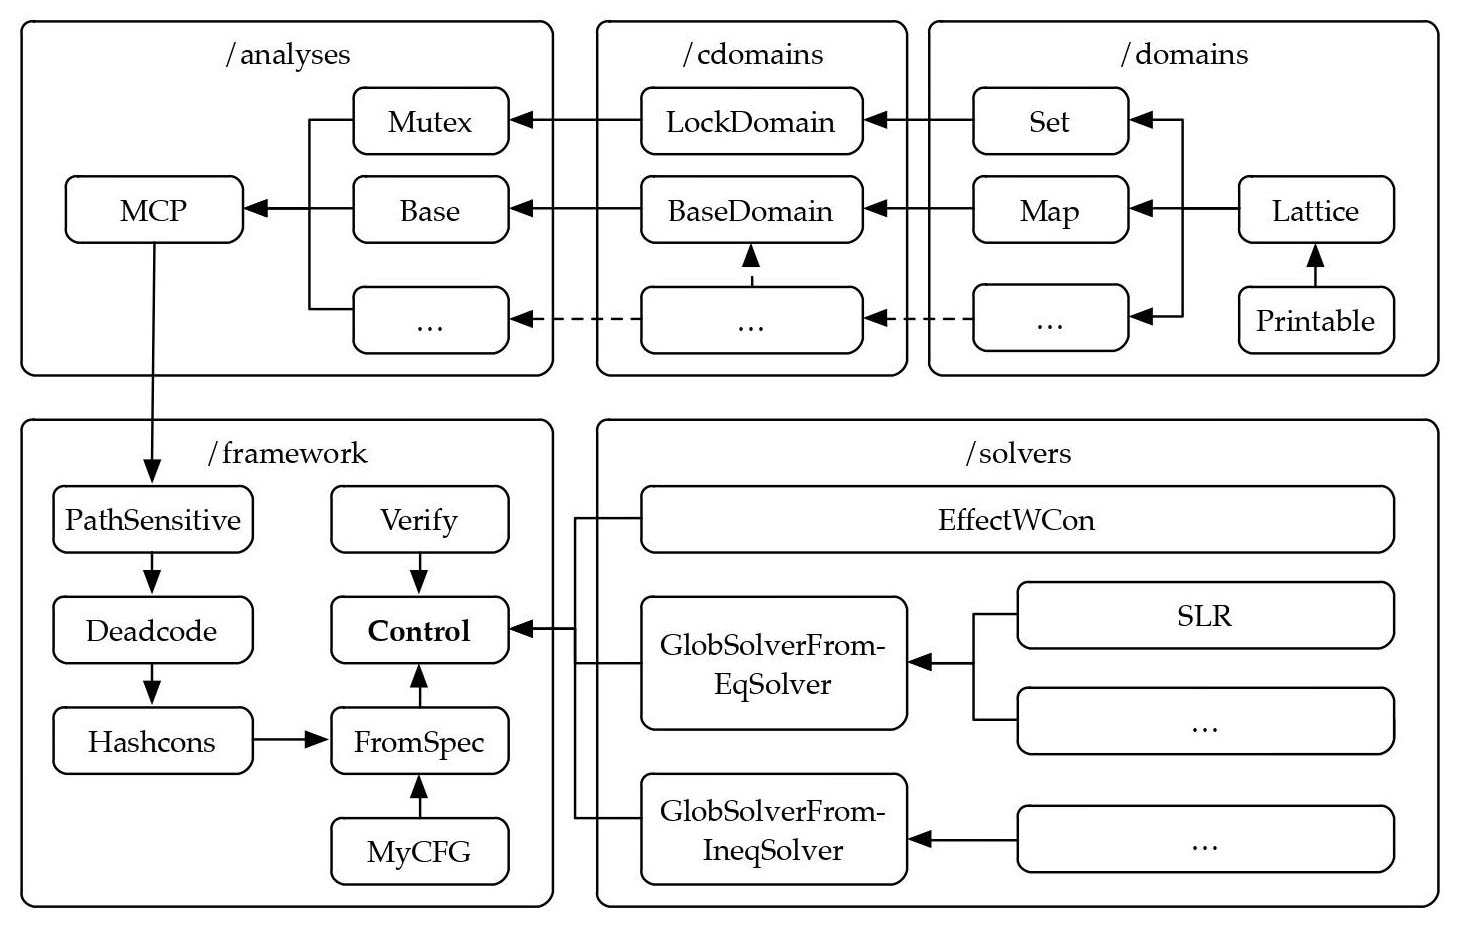
\includegraphics{../figures/goblint_structure_detailed.jpg}
      \caption{Schematic directory structure of \gob. Adapted from \parencite{apinis2014frameworks}}
      \label{fig:gob_structure_detail}
    \end{figure}

    \begin{figure}
      \centering
      \lstinputlisting[language={[Objective]Caml}]{../code/analyses.ml}
      \caption{Simplified Interface for implementing analyses in \gob}
      \label{fig:analysis_interface}
      %TODO: reference github for this file
    \end{figure}



  -- Full New Section: ThreadCreate analysis

% !TeX root = ../main.tex
% Add the above to each chapter to make compiling the PDF easier in some editors.

\chapter{Evaluation}\label{chapter:evaluation}
  
  \section{Testing}
  % TODO: Is Taint analysis sound?
  
  \section{Benchmarking}
  % TODO: Does Taint analysis actually improve overall Analysis? Speed/accuracy vs. ctxinsens/ctxsens
% !TeX root = ../main.tex
% Add the above to each chapter to make compiling the PDF easier in some editors.

\chapter{Conclusion}\label{chapter:conclusion}
% TODO: What are the overall results?



\appendix{}
Abbreviations % TODO: Abbreviations
\begin{itemize}
  \item CFG
\end{itemize}

\microtypesetup{protrusion=false}
\listoffigures{}
\listoftables{}
\microtypesetup{protrusion=true}
\printbibliography{}

\end{document}
